\chapter{Plataforma de desarrollo}
\label{cap:capitulo3}


La herramienta que se ha utilizado para el desarrollo tanto hardware como software es Arduino. Arduino es una plataforma electrónica de código abierto basada en hardware y 
software fáciles de usar. Las placas Arduino son capaces de leer entradas (la luz de un sensor, un dedo sobre un botón o un mensaje de Twitter) y convertirlas en salidas 
(activar un motor, encender un LED, publicar algo en Internet). Puedes decirle a tu placa lo que tiene que hacer enviando una serie de instrucciones al 
microcontrolador de la placa. Para ello se utiliza el lenguaje de programación Arduino (basado en Wiring) y el software Arduino (IDE), basado en Processing.

\vspace{1cm}

\begin{figure} [h!]
    \begin{center}
      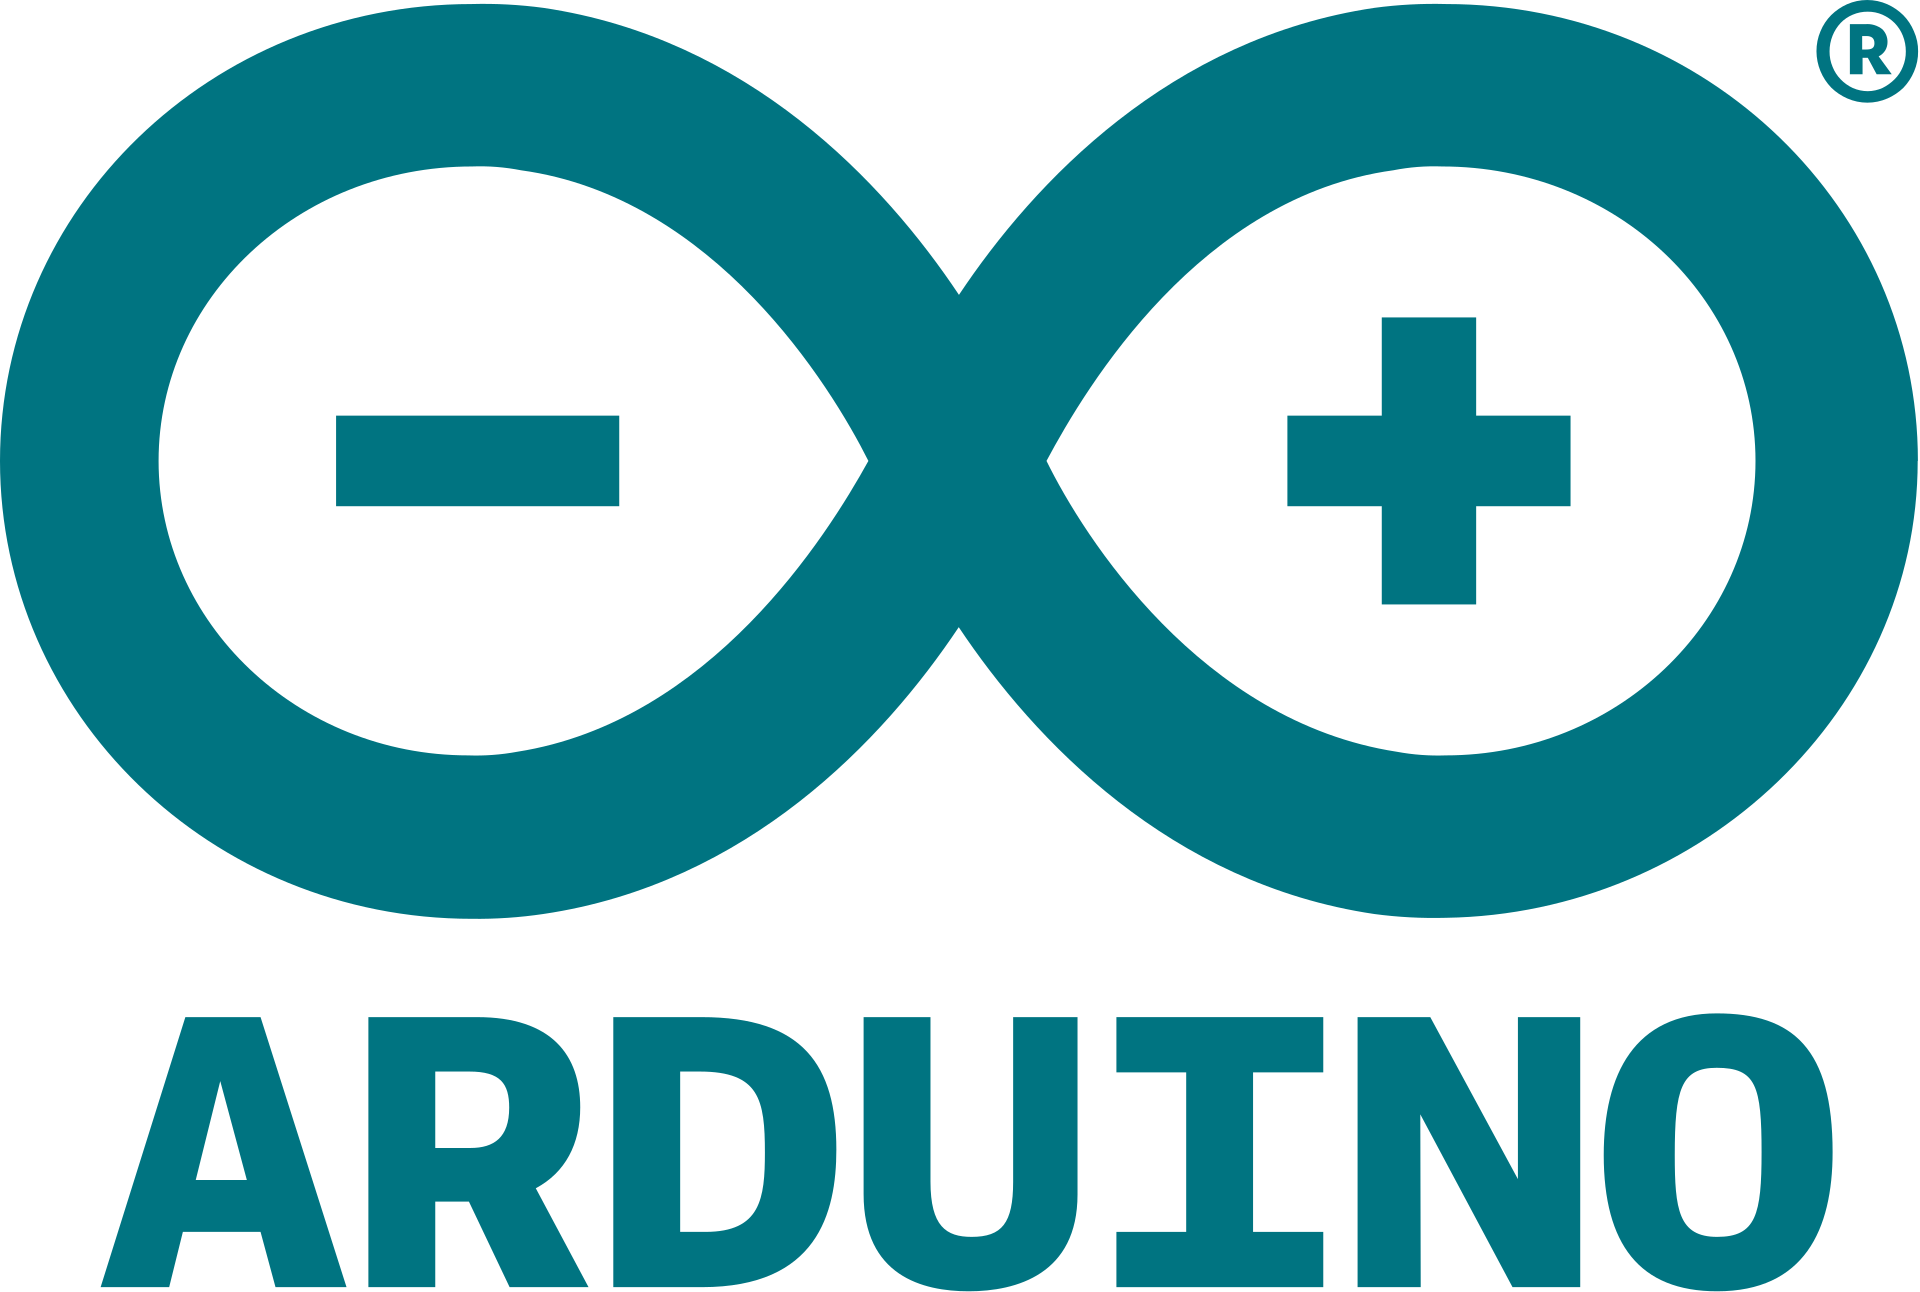
\includegraphics[width=8cm]{figs/arduino}
    \end{center}
    \caption{Logo de Arduino.}
    \label{fig:arduino}
  \end{figure}\

  Arduino nació en el  IDII (Ivrea Interaction Design Institute) como una herramienta sencilla para la creación rápida de prototipos, dirigida a estudiantes sin conocimientos previos 
  de electrónica y programación. Tan pronto como llegó a una comunidad más amplia, la placa Arduino empezó a cambiar para adaptarse a nuevas necesidades y retos, diferenciando 
  su oferta de simples placas de 8 bits a productos para aplicaciones IoT, wearables, impresión 3D y entornos embebidos.

  